\begin{figure}
%\begin{subfigure}[b]{0.33\textwidth}
%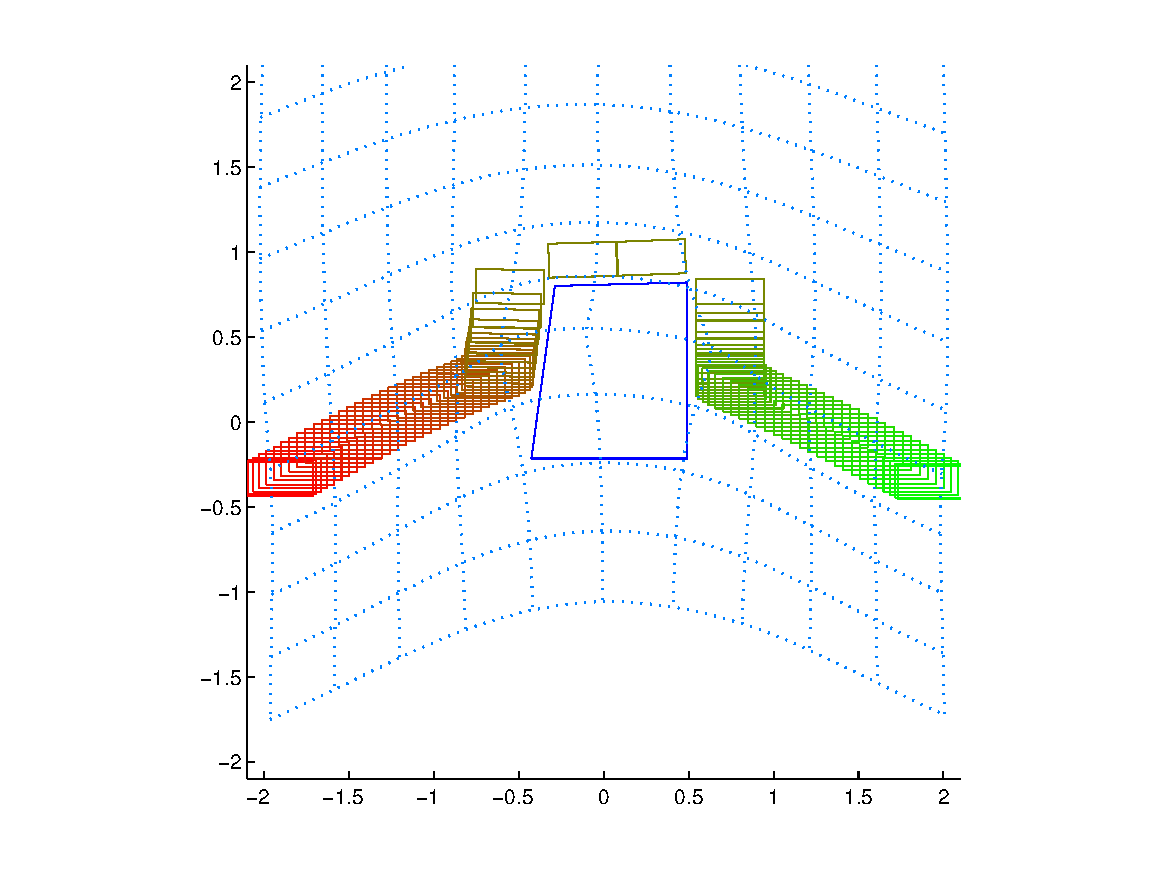
\includegraphics[width=\textwidth]{holonomic_twostep}
%\caption{}
%\end{subfigure}
\begin{subfigure}[b]{0.33\textwidth}
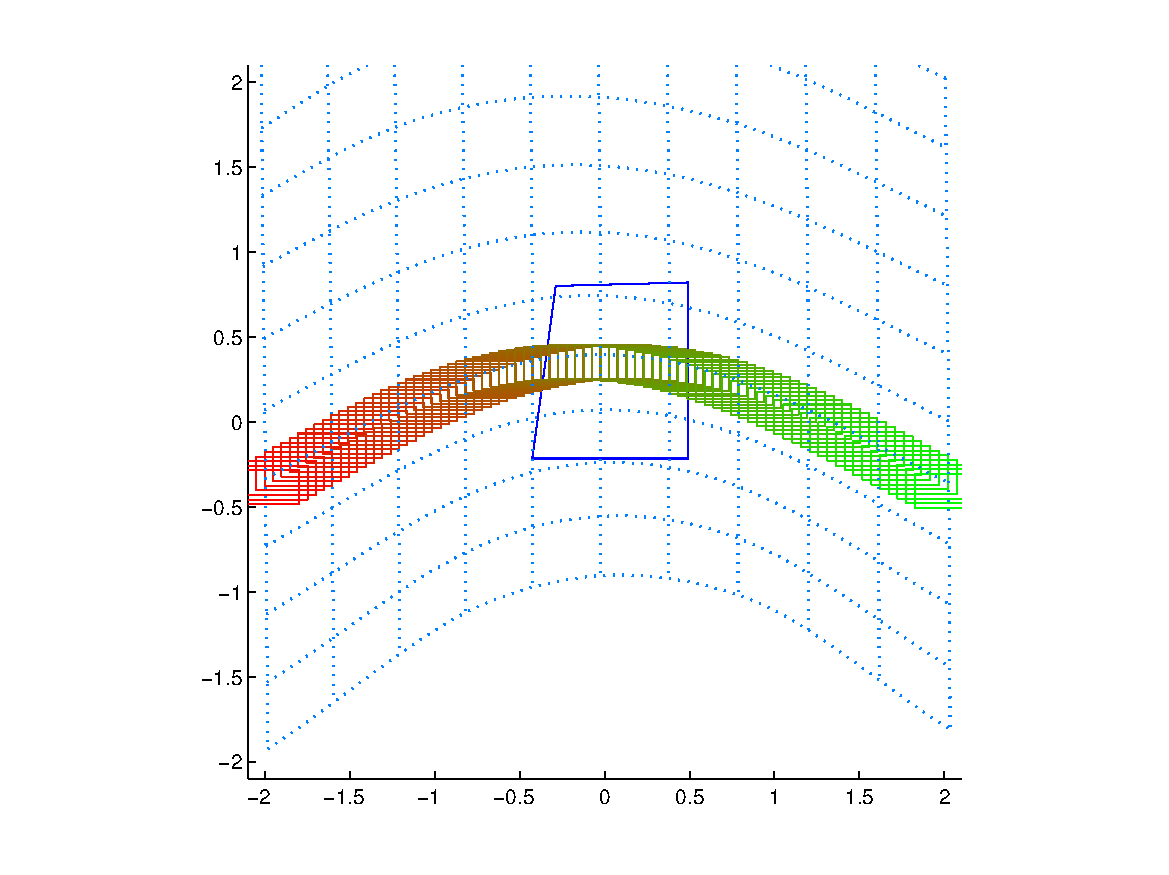
\includegraphics[width=\textwidth]{holonomic_warponly}
\caption{Registration error: 0.1957}
\label{subfig:holonomic_results_warponly}
\end{subfigure}
\begin{subfigure}[b]{0.33\textwidth}
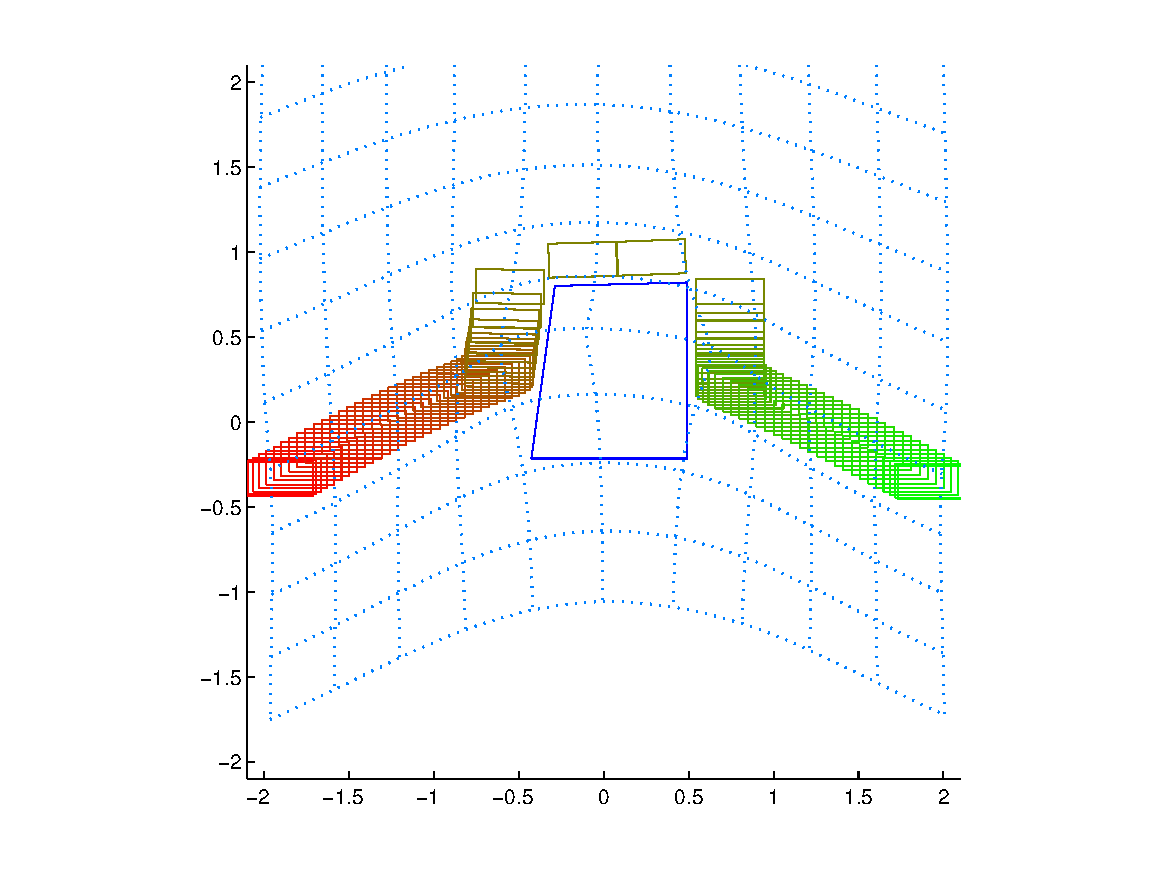
\includegraphics[width=\textwidth]{holonomic_twostep}
\caption{Registration error: 1.2323}
\label{subfig:holonomic_results_twostep}
\end{subfigure}
\begin{subfigure}[b]{0.33\textwidth}
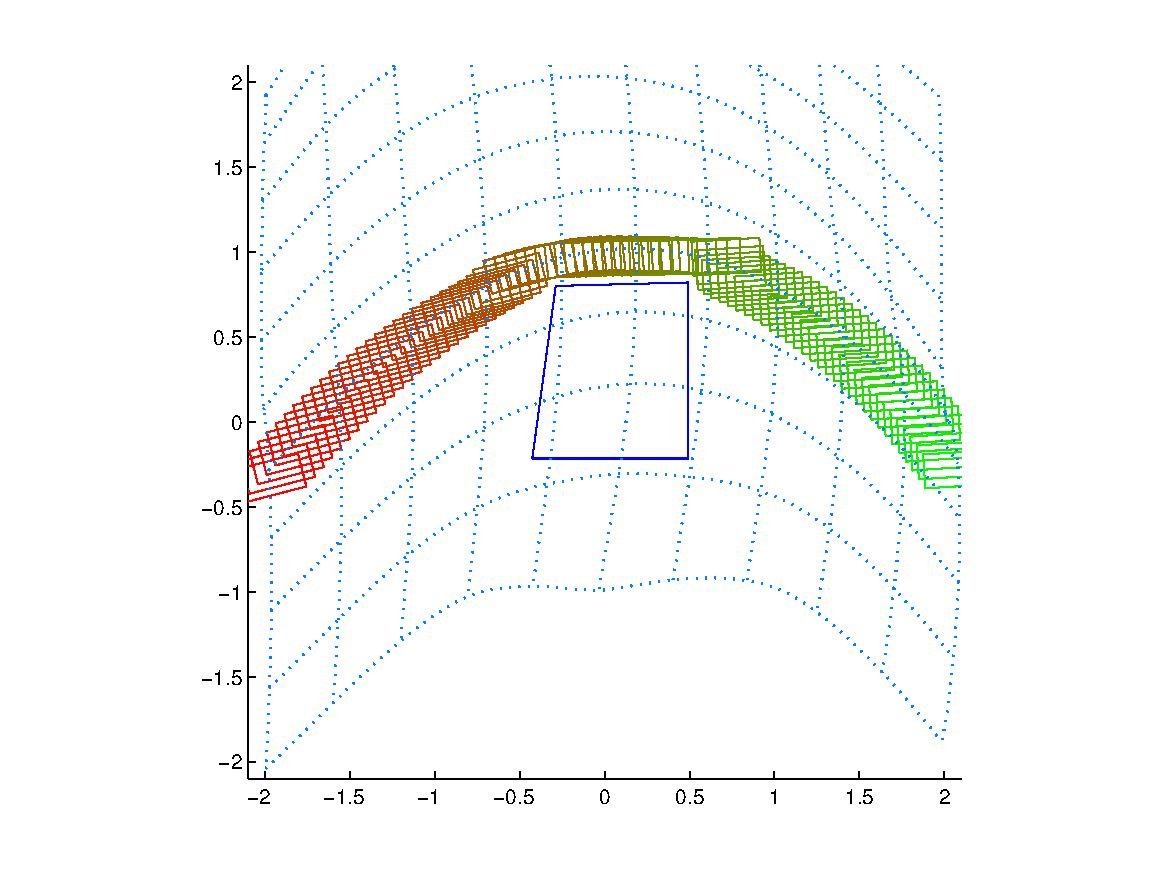
\includegraphics[width=\textwidth]{holonomic_unified}
\caption{Registration error: 0.2146}
\label{subfig:holonomic_results_unified}
\end{subfigure}
\caption{We qualitatively compared the two-step optimization method to our unified optimization method in a holonomic car example, in which a new obstacle is introduced at test time. (a): The resulting trajectory before feasibility constraints are enforced. (b): The old, two-step method produces a trajectory that poorly navigates the new obstacle. (c): Unified optimization produces a trajectory that smoothly avoids the obstacle.}
\label{fig:holonomic_results}
\end{figure}

\begin{figure}
\centering
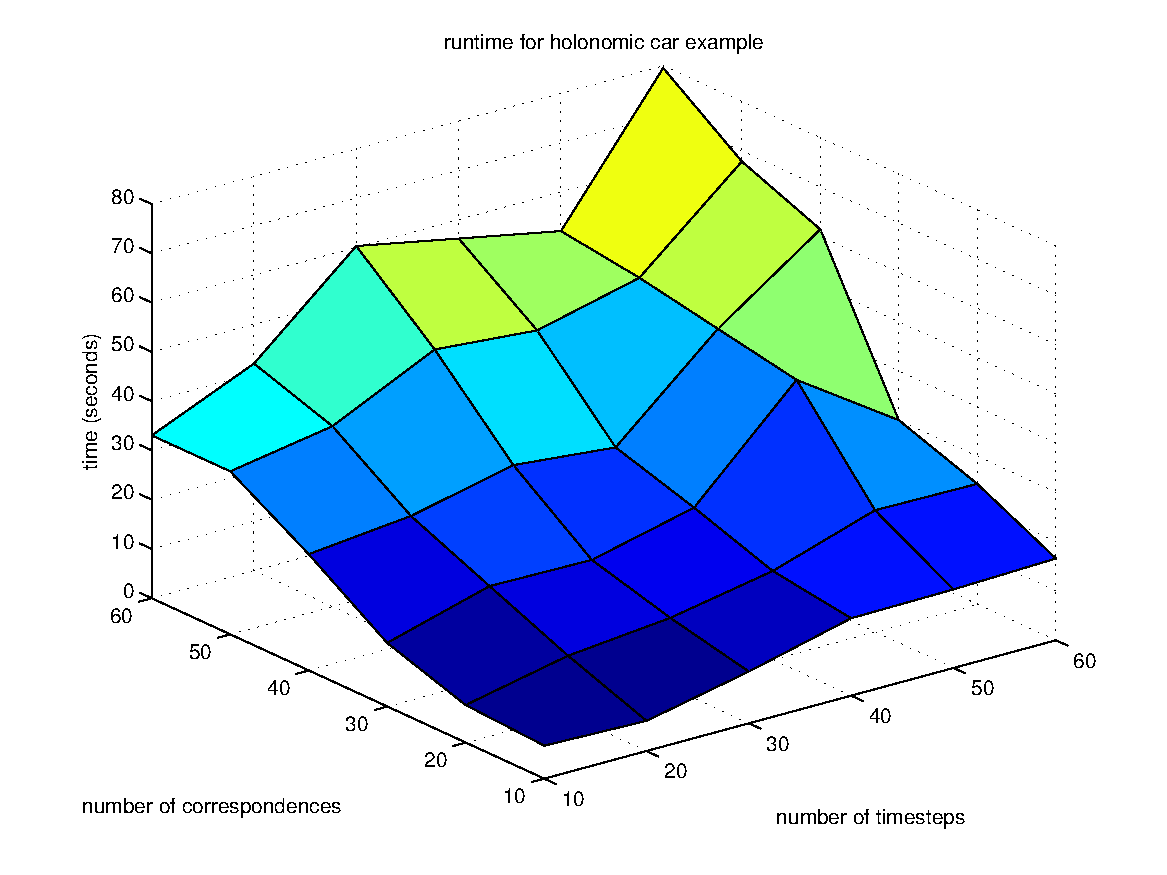
\includegraphics[width=0.7\textwidth]{holonomic_runtime}
\caption{A plot of the runtime of the holonomic car example as the number of correspondences and the number of trajectory timesteps vary.}
\label{fig:holonomic_runtime}
\end{figure}

Our unified optimization leads to improved performance over the two-step appraoch on two-dimensional tasks with pre-defined scene correspondences. We evaluated our unified optimization on a two-dimensional holonomic car example. The demonstration trajectory simply drives from left to right in a straight line. However, the ground-truth warp for the test scene bends the trajectory upwards and introduces an obstacle in the middle of the scene, such that the trajectory is blocked, as in Figure~\ref{subfig:holonomic_results_warponly}. The two-step approach, shown in Figure~\ref{subfig:holonomic_results_twostep}, poorly navigates around the obstacle, following its boundary closely. On the other hand, the unified optimization, shown in Figure~\ref{subfig:holonomic_results_unified}, smoothly navigates around the obstacle. This occurs because the unified optimization can alter the warp slightly to direct the trajectory \emph{above} the obstacle, rather than attempting to pass through it. We feel that this qualitatively demonstrates that the unified optimization produces better-conditioned trajectories.

We also performed a short experimental runtime analysis on this example. Figure~\ref{fig:holonomic_runtime} shows a plot of the runtime as we vary the number of timesteps in the trajectory and the number of scene correspondences. We find that adding additional correspondences has a much more significant effect on the runtime, since each additional correspondence greatly increases the size of the optimization problem.
